\documentclass[11pt,a4paper]{article}

% Pacotes essenciais
\usepackage[utf8]{inputenc}
\usepackage[T1]{fontenc}
\usepackage{lmodern}
\usepackage[portuguese]{babel}
\usepackage{graphicx}
\usepackage{amsmath}
\usepackage{amsfonts}
\usepackage{amssymb}
\usepackage{float}
\usepackage{caption}
\usepackage{subcaption}
\usepackage{xcolor}
\usepackage{fancyhdr}
\usepackage{geometry}
\usepackage{titlesec}

\usepackage{cite}
\usepackage{booktabs}
\usepackage{array}
\usepackage{tikz}
\usepackage[hidelinks]{hyperref}

% Definição das cores
\definecolor{headercolor}{HTML}{b11116}
\definecolor{secondarycolor}{HTML}{3a5461}

% Configuração da página
\geometry{
    a4paper,
    top=2.8cm,
    bottom=2.5cm,
    left=2.5cm,
    right=2.5cm,
    headheight=1.2cm,
    headsep=0.5cm
}

% Configuração do cabeçalho
\pagestyle{fancy}
\fancyhf{}
\renewcommand{\headrulewidth}{0pt}
\renewcommand{\footrulewidth}{0.5pt}

\fancyhead[L]{%
    \begin{tikzpicture}[remember picture, overlay]
        \fill[headercolor] (current page.north west) rectangle ([yshift=-1.2cm]current page.north east);
        \node[anchor=west, inner sep=0pt] at ([xshift=1cm, yshift=-0.6cm]current page.north west) 
            {
\includegraphics[height=0.8cm]{imgs/base/fatec-rgt.png}};
        \node[anchor=east, inner sep=0pt] at ([xshift=-1cm, yshift=-0.6cm]current page.north east) 
            {
\includegraphics[height=0.9cm]{imgs/base/cps-logo.png}};
        \node[anchor=east, inner sep=0pt] at ([xshift=-2.8cm, yshift=-0.6cm]current page.north east) 
            {
\includegraphics[height=1.05cm]{imgs/base/governo-sp-secretaria-logo.png}};
    \end{tikzpicture}
}

\fancyfoot[L]{\footnotesize\textcolor{secondarycolor}{Faculdade de Tecnologia do Estado de São Paulo\\ fatecregistro.cps.sp.gov.br}}
\fancyfoot[R]{\thepage}

% Configuração dos títulos das seções
\titleformat{\section}  
    {\normalfont\large\bfseries\color{secondarycolor}}
    {\thesection}{1em}{}

\titleformat{\subsection}
    {\normalfont\normalsize\bfseries\color{secondarycolor}}
    {\thesubsection}{1em}{}

% Informações do artigo
\title{\vspace{0.6cm}\textbf{\large Criação de Camarão em Cativeiro com Monitoramento IoT para Gastronomia} \\[0.2cm]
\large \textit{Shrimp Farming in Captivity with IoT Monitoring for Gastronomy}}

\author{
    Davi Mathais de Almeida$^{1}$, Leandro Augusto Muniz$^{1}$, Tiago de Lara Rodrigues$^{1}$ \\[0.3cm]
    \small
    $^{1}$Faculdade de Tecnologia do Estado de São Paulo \\
    \textit{davi.almeida@aluno.cps.sp.gov.br, leandro.muniz@aluno.cps.sp.gov.br,} \\
    \textit{tiago.rodrigues01@aluno.cps.sp.gov.br}
}
\date{}

\begin{document}

% Força o cabeçalho em todas as páginas
\pagestyle{fancy}

\maketitle
\thispagestyle{fancy}

% Resumo
\section*{Resumo}

A carcinicultura no Vale do Ribeira, em São Paulo, apresenta elevado potencial produtivo, mas enfrenta desafios relacionados ao manejo predominantemente manual e à falta de infraestrutura tecnológica. Para mitigar esses problemas, este trabalho propõe o desenvolvimento de um sistema de monitoramento inteligente e automação para cativeiros de camarão, integrando Internet das Coisas (IoT) a uma Aplicação Web Progressiva. O sistema utiliza um microcontrolador ESP32 equipado com sensores para coleta em tempo real de temperatura, pH e amônia, além de um dispensador automatizado de ração. Os dados são enviados para um banco de dados em nuvem e disponibilizados em um painel interativo que oferece histórico em gráficos e controle remoto. Testes de validação realizados em ambiente real, com camarões em aquário, demonstraram alta precisão do sensor de temperatura (98,27\%) e desempenho satisfatório do sensor de pH (95,98\%), embora o sensor de amônia e o mecanismo do alimentador tenham apresentado limitações operacionais. Conclui-se que a solução possui viabilidade técnica para auxiliar produtores no acompanhamento contínuo da qualidade da água, promovendo uma gestão mais eficiente, com aprimoramentos futuros direcionados à robustez dos componentes.

\vspace{0.3cm}
\noindent\textit{\textbf{Palavras-chave:}} Carcinicultura, Monitoramento, Internet das Coisas, Automação, Vale do Ribeira.

\section*{Abstract}

Shrimp farming in the Vale do Ribeira, São Paulo, has high productive potential but faces challenges related to predominantly manual management and a lack of technological infrastructure. To mitigate these problems, this work proposes the development of an intelligent monitoring and automation system for captive shrimp farming, integrating the Internet of Things (IoT) with a Progressive Web Application. The system uses an ESP32 microcontroller equipped with sensors for real-time collection of temperature, pH, and ammonia, in addition to an automated feed dispenser. Data is sent to a cloud database and made available on an interactive dashboard that offers historical graphs and remote control. Validation tests conducted in a real environment, with shrimp in an aquarium, demonstrated high accuracy of the temperature sensor (98.27\%) and satisfactory performance of the pH sensor (95.98\%), although the ammonia sensor and the feeder mechanism presented operational limitations. It is concluded that the solution is technically viable to assist producers in the continuous monitoring of water quality, promoting more efficient management, with future improvements directed towards the robustness of the components.

\vspace{0.3cm}
\noindent\textit{\textbf{Keywords:}} Shrimp farming, Monitoring, Internet of Things, Automation, Vale do Ribeira.

\vspace{0.5cm}
\noindent\rule{\textwidth}{0.5pt}
\vspace{0.5cm}

% Introdução
\section{Introdução}

Segundo \cite{bertini2021}, Caridea é um grupo de crustáceos amplamente conhecido como camarões, animais da ordem Decapoda, encontrados em ambientes de água doce ou salgada. Estima-se a existência de aproximadamente 3.500 espécies, distribuídas em 16 superfamílias e 36 famílias, sendo cerca de 800 de água doce e 2.700 de água salgada. A carcinicultura refere-se à criação de camarões em viveiros, podendo ser aplicada a espécies marinhas ou de água doce.

A produção mundial de camarão tem crescido, em média, 4,97\% ao ano nos últimos sete anos, com o Equador como maior produtor e exportador, seguido por China, Índia, Vietnã, Indonésia, Tailândia e Brasil \cite{CamaraoBrasileiro2025, Rocha2024}.  No Brasil, o camarão é a segunda maior fonte de valor na produção aquícola, concentrando-se principalmente na região Nordeste, com destaque para o Ceará, que registrou 43,7 mil toneladas em 2022. A região Nordeste responde por cerca de 99\% da produção brasileira, totalizando 92,4 mil toneladas no mesmo ano \cite{Ximenes2023}.

O Vale do Ribeira, localizado no sul do estado de São Paulo, apresenta condições ambientais favoráveis à carcinicultura, como rios, estuários e manguezais, com produção concentrada nos municípios de Cananeia, Eldorado e Sete Barras. Os carídeos de água doce da região pertencem às famílias Palaemonidae e Atyidae, com destaque para os gêneros \textit{Palaemon}, \textit{Palaemonetes} e \textit{Macrobrachium} \cite{bertini2021}. Apesar do potencial produtivo, a atividade enfrenta desafios relacionados à má gestão dos tanques, infraestrutura limitada, poluição e proliferação de doenças, comprometendo a qualidade do produto e a rentabilidade.

A qualidade da água é um dos fatores determinantes para a produção de camarões com valor gastronômico. Parâmetros como temperatura, potencial hidrogeniônico e amônia exercem influência direta sobre o desenvolvimento, o bem-estar e as características sensoriais dos animais, como textura, sabor e odor do produto final \cite{Embrapa2023}. Alterações fora das faixas ideais comprometem não apenas a saúde dos camarões, mas também a aceitação do produto pelo consumidor e sua competitividade no mercado gastronômico, que exige padrões cada vez mais rigorosos de rastreabilidade e qualidade. Nesse contexto, o monitoramento contínuo e preciso das condições do cativeiro torna-se indispensável para garantir a produção de um camarão com qualidade adequada para fins gastronômicos, objetivo central deste trabalho.

Para entender as condições reais de manejo na região, foi conduzida uma pesquisa de campo com participantes vinculados à carcinicultura no Vale do Ribeira, por meio de entrevistas estruturadas com roteiro de dez questões voltadas às rotinas de manejo e aos cuidados com os cativeiros. Os resultados indicaram que o manejo é realizado de forma predominantemente manual, com os responsáveis dedicando em média cinco horas diárias ao cuidado dos cativeiros e realizando a verificação dos parâmetros da água de três a quatro vezes por dia, nos períodos da manhã, tarde e noite. Os participantes relataram que já ocorreram perdas de camarões tanto por falhas na alimentação, situações em que os animais deixaram de ser alimentados, quanto por alterações nos parâmetros da água, especialmente elevação da amônia, que se converte em nitrito e compromete a qualidade do ambiente aquático. A ausência de controle automatizado da alimentação e de registro histórico dos parâmetros ambientais foi apontada como principal fator que dificulta a identificação precoce de alterações críticas e aumenta o risco de perdas.

Nesse contexto, a Internet das Coisas tem se consolidado como uma abordagem promissora para o monitoramento e automação de sistemas aquícolas. A capacidade de coletar dados ambientais em tempo real por meio de sensores conectados, transmiti-los para a nuvem e disponibilizá-los ao produtor de forma remota representa um avanço significativo em relação ao manejo manual tradicional. Estudos recentes demonstram que a adoção de sistemas baseados em IoT na carcinicultura contribui para o aumento da precisão no monitoramento da qualidade da água, a redução do tempo de resposta a alterações críticas e a melhoria dos indicadores produtivos, como taxa de sobrevivência e crescimento dos animais \cite{Uddin2020, Zainuddin2019}. A integração dessas tecnologias à realidade dos produtores do Vale do Ribeira representa, portanto, uma oportunidade concreta de modernização da atividade com impacto direto na qualidade e na rentabilidade da produção.

Para superar esses desafios, é proposta a implementação de um sistema de monitoramento inteligente baseado em Internet das Coisas (do inglês, \textit{Internet of Things}, ou IoT). O sistema monitora parâmetros críticos, como temperatura, potencial hidrogeniônico (pH) e amônia, utilizando sensores conectados ao microcontrolador ESP32 com rede sem fio (\textit{Wi-Fi}) para coleta e transmissão de dados em tempo real. A aplicação web permite ao usuário visualizar informações, controlar remotamente as operações e acionar um alimentador automático programável, que distribui ração conforme horários e quantidades definidas. Além disso, o sistema gera relatórios históricos, gráficos e envia notificações preventivas em caso de alterações críticas, garantindo maior eficiência e segurança na criação de camarões.

% Objetivo
\section{Objetivos}

Este trabalho tem como objetivo desenvolver um sistema de monitoramento automatizado para cativeiros de camarão, integrando sensores IoT a uma aplicação web progressiva, a fim de auxiliar produtores no acompanhamento contínuo dos parâmetros ambientais e no controle da alimentação dos cativeiros.

\subsection{Objetivos específicos}

\begin{enumerate}
    \item Monitorar remotamente os parâmetros de temperatura, pH e amônia da água dos cativeiros, emitindo alertas automáticos ao usuário em caso de desvios nos valores esperados.

    \item Registrar e armazenar dados históricos dos cativeiros, disponibilizando relatórios e gráficos para análise das condições ambientais ao longo do tempo.

    \item Automatizar o fornecimento de ração por meio de um dispensador controlado pelo sistema, com definição de horários e quantidades pelo usuário.
    
    \item Desenvolver uma aplicação web responsiva disponibilizando ao produtor acesso remoto em tempo real aos parâmetros monitorados e aos controles de alimentação dos cativeiros, sem necessidade de instalação nativa.

\end{enumerate}

% Estado da Arte
\section{Estado da Arte}

A utilização de sistemas de monitoramento baseados em IoT na carcinicultura tem sido explorada em diferentes contextos, com abordagens variadas quanto à tecnologia de comunicação, aos parâmetros monitorados e à forma de suporte à decisão.

O trabalho de \cite{dantas2020} propõe um sistema de telemonitoramento para a criação de camarões utilizando microcontroladores ESP32 integrados a módulos de Longo Alcance (do inglês, \textit{Long Range}, ou LoRa) e sensores de pH, oxigênio dissolvido e temperatura. A transmissão dos dados ocorre via Rede de Longo Alcance e Ampla Cobertura (do inglês, \textit{Long Range Wide Area Network}, ou LoRaWAN), com integração aos Serviços de Nuvem da Amazon (do inglês, \textit{Amazon Web Services}, ou AWS) por meio do Protocolo de Telemetria por Enfileiramento de Mensagens (do inglês, \textit{Message Queuing Telemetry Transport}, ou MQTT). A escolha do LoRaWAN foi motivada pela necessidade de cobrir grandes áreas rurais sem dependência de infraestrutura de rede local. Os resultados apresentaram medições precisas de temperatura e pH, com variações mínimas de 0,5°C, e alcance de comunicação de aproximadamente 138 metros, suficiente para fazendas de pequeno e médio porte. As principais limitações foram a necessidade de ampliação do alcance para fazendas maiores, o aprimoramento da autonomia energética e a inclusão de sensores adicionais, como amônia e turbidez.

\cite{Uddin2020} apresenta um sistema de monitoramento em tempo real para fazendas de camarão de água doce (\textit{Macrobrachium rosenbergii}) em Bangladesh, integrando sensores de temperatura, pH, salinidade, oxigênio dissolvido e turbidez a um microcontrolador Arduino Yun. Os dados são transmitidos para uma camada de nuvem que aplica o método de Análise Hierárquica (do inglês, \textit{Analytic Hierarchy Process}, ou AHP), calculando um índice composto de qualidade da água que orienta o produtor sobre a necessidade de intervenção, com notificações automáticas via portal web. O sistema operou por 120 dias em ambiente real de cultivo, coletando mais de 4.600 registros com erro médio inferior a 7\% em relação a medições manuais de referência. A comparação entre um tanque monitorado pelo sistema IoT e outro gerenciado manualmente evidenciou ganhos expressivos: comprimento médio de 9 a 12 cm contra 8 a 10 cm, peso de 20 g contra 17 g e taxa de sobrevivência de 90\% contra 80--90\%. Como limitações, os autores apontam a dependência de conectividade Wi-Fi, a necessidade de calibração periódica dos sensores e desafios de escalabilidade para fazendas de grande porte.

\cite{Zainuddin2019} propõem um sistema de monitoramento da qualidade da água em viveiros de camarão vannamei (\textit{Litopenaeus vannamei}), estruturado com base em uma Rede de Sensores Sem Fio (do inglês, \textit{Wireless Sensor Network}, ou WSN). Sensores de temperatura DS18B20, pH e turbidez foram distribuídos em cinco pontos estratégicos do viveiro, conectados a microcontroladores Atmega 2560 e Atmega 328, com comunicação via módulos Xbee (protocolo Zigbee) e transmissão para uma aplicação web por meio do ESP8266. A calibração com instrumentos de referência resultou em acurácia de 97,75\% para temperatura, 98,85\% para pH e 99,73\% para turbidez. A arquitetura distribuída da WSN representa o principal diferencial, permitindo cobertura espacial simultânea de múltiplos pontos do viveiro. As limitações incluem instabilidade na transmissão em condições de conectividade deficiente, restrições na expansão para novos sensores e ausência de mecanismos de redundância.

Os três trabalhos analisados compartilham o foco no monitoramento remoto de parâmetros da água por meio de IoT, demonstrando a viabilidade da abordagem para a carcinicultura, mas apresentando limitações comuns relacionadas à conectividade, escalabilidade e calibração. Nenhum dos sistemas avaliados integra o controle automatizado da alimentação ao monitoramento ambiental, tratando essas duas funções como responsabilidades separadas do produtor. Em comparação, o sistema proposto neste trabalho diferencia-se por integrar o monitoramento de temperatura, pH e amônia ao controle automatizado da alimentação, com definição de horários e quantidades de ração, geração de relatórios e gráficos históricos e envio de alertas preventivos, unificando monitoramento ambiental, controle alimentar e apoio à gestão em uma única solução voltada à realidade do Vale do Ribeira.

% Metodologia
\section{Metodologia}

O sistema foi desenvolvido seguindo uma abordagem iterativa, com ciclos de desenvolvimento, teste e refinamento realizados ao longo do projeto. O projeto foi estruturado em duas frentes de desenvolvimento: a aplicação web e o componente IoT. A aplicação web foi estruturada em duas camadas: a interface de usuário, implementada no modelo de Aplicativo Web Progressivo (do inglês, \textit{Progressive Web App}, ou PWA) com o framework Next.js 14, baseado na biblioteca React 18, garantindo acesso via dispositivos móveis sem necessidade de instalação nativa; e a camada de servidor, construída com Node.js e o framework Express, responsável pelo gerenciamento de dados, autenticação de usuários por meio de Tokens de Autenticação (do inglês, \textit{JSON Web Token}, ou JWT) e comunicação com os equipamentos de monitoramento. Os dados coletados são armazenados em banco de dados MongoDB, solução não relacional que permite armazenamento flexível e escalável, hospedado na plataforma MongoDB Atlas. A interface de usuário foi disponibilizada na plataforma Vercel, enquanto o servidor e a interface de programação de aplicações (do inglês, \textit{Application Programming Interface}, ou API) foram hospedados no Render.

\subsection{Desenvolvimento IoT}

O componente IoT foi desenvolvido com base no microcontrolador ESP32, que atua como unidade central de processamento e comunicação. A ele foram integrados: o sensor de temperatura DS18B20, conectado ao pino de entrada digital do ESP32 por meio de resistor de pull-up; o módulo sensor de pH Ph4502, com saída analógica conectada ao conversor analógico-digital (ADC) do ESP32; o sensor de gases tóxicos modelo MQ-135, responsável pela detecção de amônia, com saídas digital e analógica também conectadas ao ADC; e o módulo relé de 5V, acionado por sinal digital do ESP32 para controle do servo motor do dispensador de ração. A alimentação do sistema é realizada via cabo de alimentação, utilizando o pino VIN para alimentar o motor com 5V e o pino 3V3 para os sensores, com referência de terra (GND) compartilhada entre todos os módulos. O esquema de ligação dos componentes é apresentado na Figura \ref{fig:iot_diagrama}. 

\begin{figure}[H]
\centering
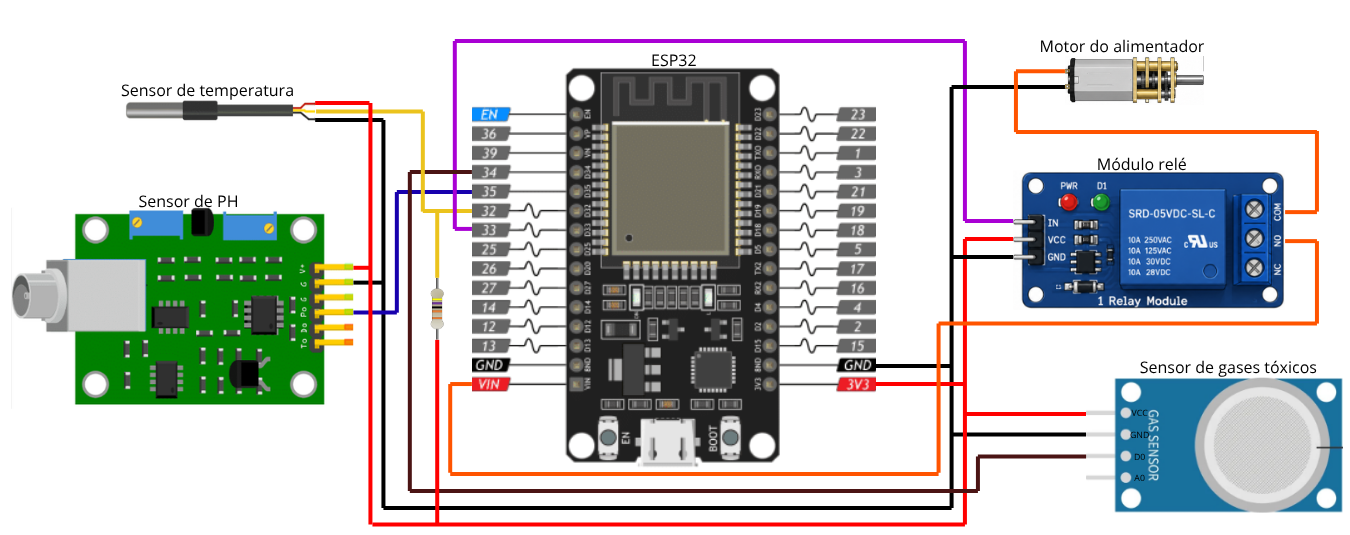
\includegraphics[width=1.0\linewidth]{imgs/diagrama-iot-camarize.png}
\caption{Diagrama referente a montagem do componente IoT}
\label{fig:iot_diagrama}
\end{figure}

O ciclo de leitura dos parâmetros e a transmissão dos pacotes via rede sem fio para a nuvem ocorrem em intervalos regulares de 1 minuto, visando manter um monitoramento contínuo adequado para a análise do cativeiro. Em caso de perda de conectividade Wi-Fi, o ESP32 armazena as leituras localmente utilizando o sistema de armazenamento não volátil (do inglês, \textit{Non-Volatile Storage}, ou NVS) disponível no próprio microcontrolador, garantindo que nenhuma leitura seja perdida durante falhas temporárias de rede. Quando a conexão é restabelecida, os dados armazenados localmente são sincronizados automaticamente com o banco de dados em nuvem, assegurando a integridade do histórico de monitoramento do cativeiro.

O controle da alimentação é realizado de forma integrada entre o ESP32 e a API. No horário programado, o ESP32 consulta a API para obter a configuração de dieta ativa do cativeiro, verificando o horário e a quantidade de ração definidos pelo usuário. Com base nessa resposta, o ESP32 aciona o servo motor do dispensador, libera a quantidade configurada e envia uma confirmação à API, que registra a alimentação realizada e notifica o usuário. Essa arquitetura garante que as configurações de alimentação sejam sempre gerenciadas de forma centralizada pela aplicação, permitindo que o usuário altere horários e quantidades remotamente sem necessidade de reconfiguração física do equipamento.

\subsection{Funcionamento do projeto}

No fluxograma apresentado abaixo, é descrito o funcionamento geral do projeto. Na Figura \ref{fig:fluxograma_funcionamento} é apresentado o fluxograma geral do sistema. Na etapa 1, o usuário realiza o cadastro na plataforma. Na etapa 2, as informações são registradas e acessadas por meio do aplicativo. Na etapa 3, o aplicativo se comunica de forma bidirecional com o banco de dados na nuvem, que armazena e disponibiliza todas as informações do sistema. Na etapa 4, o banco de dados troca dados com o equipamento IoT, representado pelo ESP32, que utiliza seus sensores para captar os parâmetros de temperatura, pH e amônia do cativeiro em tempo real. Na etapa 5, o ESP32 aciona o dispensador de ração conforme os horários e quantidades definidos pelo usuário, completando o ciclo automatizado do sistema.

\begin{figure}[H]
\centering
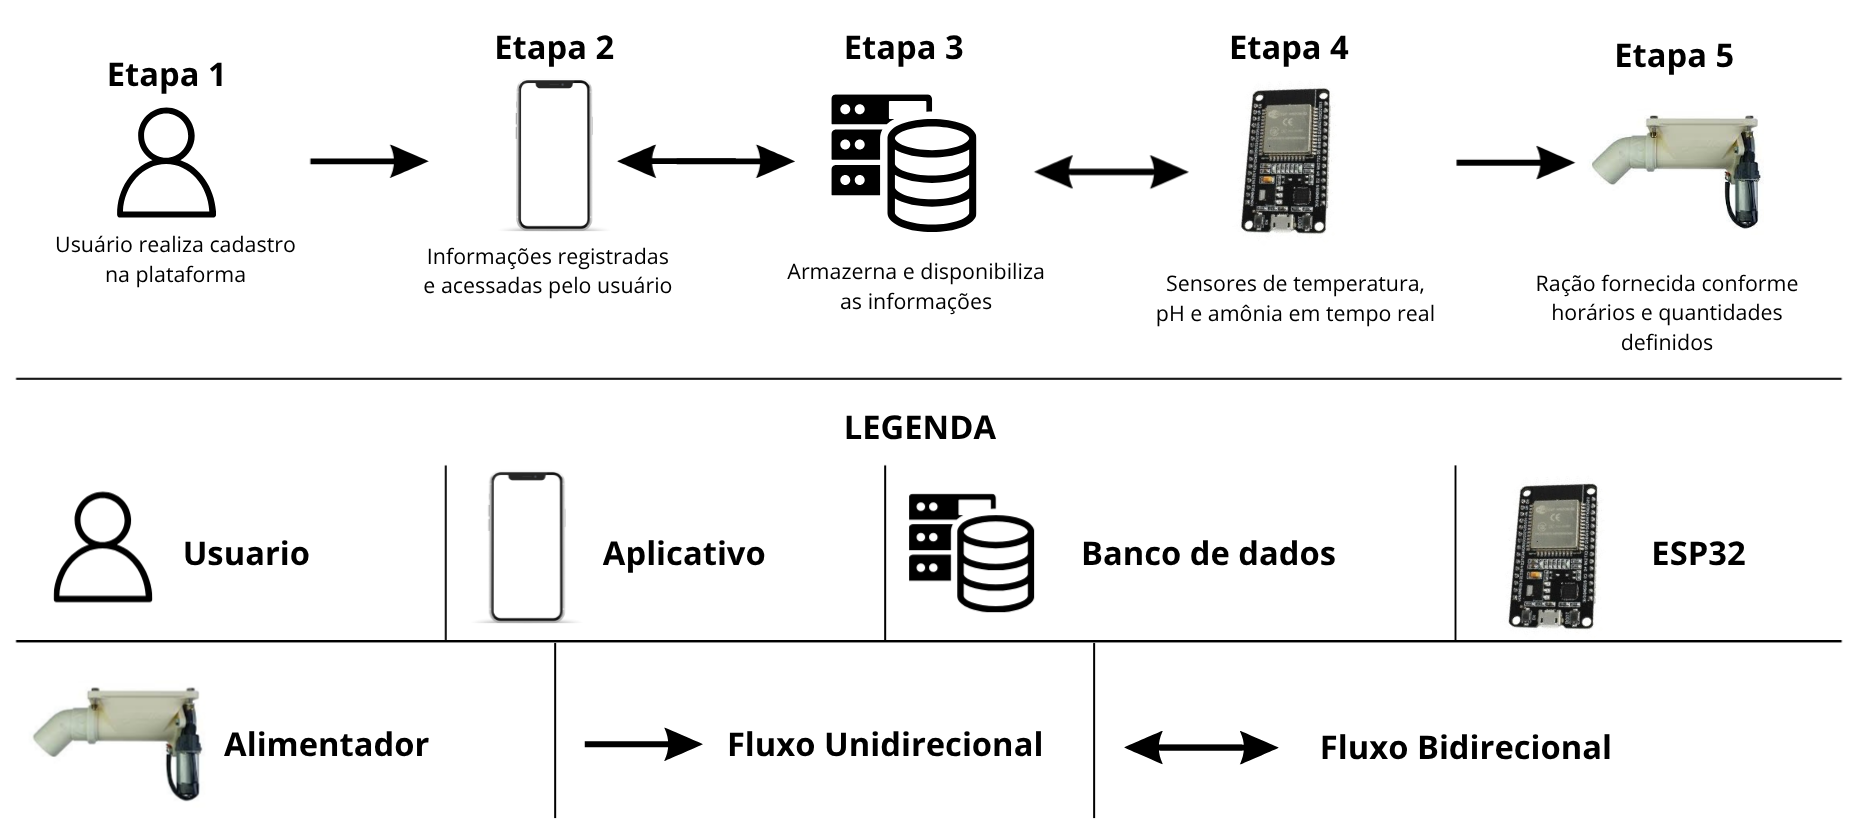
\includegraphics[width=1.0\linewidth]{imgs/fluxograma-camarize.png}
\caption{Fluxograma sobre funcionamento do sistema}
\label{fig:fluxograma_funcionamento}
\end{figure}

\subsection{Validação dos Sensores}

A validação do componente IoT foi realizada em ambiente real, com camarões em aquário, por meio de seis testes conduzidos em diferentes condições de temperatura e pH. As condições foram variadas de forma controlada ao longo dos testes, a fim de avaliar o comportamento dos sensores em cenários distintos de cultivo. Para cada teste, os valores de referência foram obtidos simultaneamente às leituras do ESP32, utilizando um termômetro de aquário, medidor de pH e amônia da marca OceanTech disponíveis no ambiente de teste, permitindo calcular o erro médio e a precisão de cada sensor. Os índices quantitativos obtidos a partir dessa metodologia de validação são detalhados e discutidos na seção subsequente.

% Resultados e Discussões
\section{Resultados e Discussões}

\subsection{Resultados da aplicação}

A aplicação web encontra-se em pleno funcionamento, disponível em ambiente de produção, com as funcionalidades de cadastro de usuários, gerenciamento de cativeiros, visualização de dados em painel de controle interativo, sistema de alertas automáticos e controle automatizado da alimentação operacionais. A interface foi desenvolvida seguindo os princípios de usabilidade mobile-first, e melhorias de design estão em curso para a versão final.

A interface da aplicação foi estruturada para oferecer ao produtor uma visão centralizada e intuitiva de seus cativeiros. A tela principal exibe todos os cativeiros cadastrados pelo usuário, permitindo a seleção individual de cada um para acesso às informações detalhadas. Ao acessar um cativeiro específico, o usuário visualiza os valores atuais de temperatura, pH e amônia coletados em tempo real pelo ESP32, acompanhados de gráficos históricos semanais que permitem identificar tendências e variações nas condições ambientais ao longo do tempo. Os limites ideais de cada parâmetro são definidos pelo próprio usuário no momento do cadastro do cativeiro, de acordo com as características da espécie cultivada e as condições locais de produção. Quando uma leitura ultrapassa os limites configurados, o sistema classifica automaticamente a severidade do desvio e aciona dois canais de alerta simultaneamente: uma notificação push enviada diretamente ao dispositivo móvel do usuário e um e-mail com os detalhes do parâmetro fora do limite, garantindo que o produtor seja informado independentemente de estar com a aplicação aberta no momento do evento.

O controle da alimentação é realizado diretamente pela plataforma, onde o usuário define a quantidade de ração e o número de alimentações diárias para cada cativeiro. Essas configurações são armazenadas no banco de dados em nuvem e consultadas pelo ESP32 nos horários programados, que aciona o servo motor do dispensador e registra cada alimentação realizada. O histórico de alimentações fica disponível na plataforma, permitindo ao produtor acompanhar se os ciclos de alimentação estão sendo executados corretamente ao longo do tempo.

O sistema contempla ainda diferentes níveis de acesso, com permissões distintas para cada perfil de usuário. O proprietário do cativeiro possui acesso completo às funcionalidades da plataforma, incluindo cadastro e gerenciamento de cativeiros, configuração de alertas e dietas, e visualização de relatórios. Funcionários cadastrados têm acesso restrito às informações operacionais, sem permissão para alterar configurações críticas do sistema. Essa estrutura de controle de acesso garante maior segurança operacional e permite que múltiplos colaboradores utilizem a plataforma sem comprometer a integridade das configurações definidas pelo proprietário.

\subsection{Validação dos sensores}

Os testes foram conduzidos considerando as faixas ideais de cultivo identificadas na pesquisa de campo, que estabelecem como valores aceitáveis: temperatura entre 25°C e 30°C, pH entre 6,5 e 8,5, e concentração de nitrito abaixo de 0,1 ppm. Essas faixas orientaram a definição dos cenários de teste e a interpretação dos resultados obtidos, uma vez que variações fora desses limites representam risco real para a saúde dos camarões em condições de produção.

O componente IoT, baseado no microcontrolador ESP32, foi submetido a uma bateria de seis testes de validação realizados em ambiente real, com camarões em aquário, utilizando instrumentos de referência para comparação simultânea das leituras. Os testes foram conduzidos em diferentes condições ambientais, variando temperatura e pH da água de forma controlada, a fim de avaliar o comportamento dos sensores em cenários distintos de cultivo. A Tabela \ref{tab:sensores} apresenta os resultados comparativos obtidos em cada teste.

\begin{table}[H]
\centering
\caption{Comparação entre valores de referência e leituras do sensor ESP32}
\resizebox{\textwidth}{!}{%
\begin{tabular}{ccccccc}
\hline
\textbf{Teste} & \textbf{Temp. Real (°C)} & \textbf{Temp. Sensor (°C)} & \textbf{pH Real} & \textbf{pH Sensor} & \textbf{Amônia Real} & \textbf{Amônia Sensor} \\
\hline
1 & 21,0 & 20,50 & 7,0 & 6,79 & 0,000 & 0,000 \\
2 & 26,0 & 25,79 & 7,0 & 6,79 & 0,000    & 0,000 \\
3 & 17,0 & 16,80 & 7,0 & 6,79 & 0,000    & 0,000 \\
4 & 21,0 & 20,50 & 5,0 & 4,80 & 0,000    & 0,000 \\
5 & 22,0 & 21,60 & 8,6 & 7,90 & 0,000    & 0,000 \\
6 & 22,0 & 21,60 & 7,0 & 6,79 & 0,000    & 0,000 \\
\hline
\textbf{Erro médio} & \multicolumn{2}{c}{\textbf{1,73\%}} & \multicolumn{2}{c}{\textbf{4,02\%}} & \multicolumn{2}{c}{—} \\
\textbf{Precisão média} & \multicolumn{2}{c}{\textbf{98,27\%}} & \multicolumn{2}{c}{\textbf{95,98\%}} & \multicolumn{2}{c}{—} \\
\hline
\end{tabular}}
\label{tab:sensores}
\end{table}

O sensor de temperatura apresentou desempenho elevado, com erro médio de 1,73\% e precisão média de 98,27\% ao longo dos seis testes, cobrindo uma faixa de variação de 17,0°C a 26,0°C. Os erros absolutos registrados foram consistentemente inferiores a 0,5°C, demonstrando estabilidade do sensor em diferentes condições térmicas. 

O sensor de pH apresentou precisão média de 95,98\%, com erro médio de 4,02\%. A análise detalhada dos resultados revela um padrão consistente: nos testes 1, 2, 3 e 6, em que o pH de referência era 7,0, o sensor registrou sistematicamente o valor de 6,79, resultando em uma diferença constante de 0,21. No teste 4, em que o pH de referência foi reduzido para 5,0, o sensor registrou 4,80, apresentando uma diferença de 0,20, praticamente idêntica à observada nos demais testes. Essa consistência do erro ao longo de diferentes faixas de pH indica que o sensor opera com um deslocamento de calibração fixo, e não com uma imprecisão aleatória ou dependente da faixa de medição. Esse comportamento sugere que um processo de recalibração pontual do sensor seria suficiente para reduzir significativamente o erro médio em todos os testes, sem necessidade de substituição do componente.

A maior divergência ocorreu no quinto teste, em que o pH foi elevado para 8,6 por meio da adição de carbonato de sódio em recipiente separado, a fim de preservar a saúde dos camarões. A medição foi realizada 30 minutos após a adição do reagente, período em que o sensor registrou 7,90 frente ao valor de referência de 8,6, resultando em uma diferença de 8,14\%, consideravelmente superior à média dos demais testes. Esse comportamento pode ser atribuído a dois fatores combinados. Primeiro, a dissolução do carbonato de sódio em água é um processo gradual que pode levar à formação de microambientes com concentrações desiguais, de modo que, mesmo após 30 minutos, a solução pode não ter atingido equilíbrio químico completo e homogeneidade. Segundo, eletrodos de pH são sensíveis a transições rápidas de alcalinidade, podendo apresentar leituras instáveis enquanto a solução ainda está em processo de homogeneização. A combinação desses dois fatores explica a divergência observada nesse teste específico e indica que, em condições estabilizadas de pH, o desempenho do sensor tende a se aproximar do padrão consistente observado nos demais testes.

O sensor de amônia registrou leitura de 0,000 ppm em todos os testes, em concordância com os valores de referência. A ausência de amônia no ambiente foi confirmada pelo fato de que o proprietário do aquário havia realizado a troca completa da água no dia dos testes, eliminando qualquer concentração residual do composto. Embora os resultados indiquem que o sensor é capaz de confirmar a ausência de amônia no ambiente, sua limitação para medições quantitativas precisas em baixas concentrações permanece identificada como ponto de melhoria, visto que o componente utilizado é um sensor de gases projetado para detecção de presença no ar, e não para quantificação em meio aquático.

O protótipo do dispensador de ração foi desenvolvido e testado, porém apresentou instabilidades mecânicas durante a operação. Com base nos resultados obtidos, o mecanismo está sendo reformulado para um modelo mais robusto, com ajustes no sistema de distribuição para garantir maior precisão e confiabilidade no ciclo de alimentação.

% Conclusão
\section{Conclusão}

O presente trabalho apresentou o desenvolvimento de um sistema integrado de monitoramento e automação para a criação de camarões em cativeiro, unindo uma aplicação web progressiva a um componente de IoT baseado no microcontrolador ESP32. A pesquisa de campo conduzida no Vale do Ribeira evidenciou a carência de tecnologia no manejo dos cativeiros da região, validando a relevância e a aplicabilidade da solução proposta.

Os resultados preliminares demonstram que a aplicação web atingiu plena funcionalidade, com todas as funcionalidades planejadas em operação. O componente IoT encontra-se em estágio avançado de desenvolvimento, com a integração dos sensores e a transmissão de dados validadas em ambiente controlado, representando aproximadamente 70\% a 80\% da implementação prevista.

Embora limitações como a dependência de conectividade Wi-Fi, a imprecisão do sensor de amônia em meio aquoso e instabilidades mecânicas no dispensador de ração tenham sido identificadas, o projeto consolida uma base tecnológica promissora. Como trabalhos futuros, planeja-se a validação completa do protótipo em ambiente real de cativeiro, a substituição do sensor de amônia por um modelo específico para água e a construção de um mecanismo de alimentação mais robusto. O projeto terá continuidade com foco na coleta de dados de longa duração, buscando entregar uma solução acessível, eficiente e sustentável para o fomento da carcinicultura no Vale do Ribeira.

% Referências
\bibliographystyle{IEEEtran}
\bibliography{referencias}

\end{document}
